%%%%%%%%%%\dir %%%%%%%%%%%%%%%%%%%%%%%%%%%%%%%%%%%%%%%%
\begin{frame}[fragile]{\de{xxx}\en{The Plan for Today}}

\begin{itemize}
\item Only 1 hour
\item Only 1 pattern
\vspace{1em}
\item Most important one for me right now
\end{itemize}

\end{frame}



%%%%%%%%%%%%%%%%%%%%%%%%%%%%%%%%%%%%%%%%%%%%%%%%%%
\begin{frame}[fragile]{\de{Was ist das Problem?}\en{What is the problem?}}

\begin{lstlisting}
public double calcDiscount( double p1, double p2 ){
   // ...
}
\end{lstlisting}

\onslide+<2->

\vspace{2em}

$\longrightarrow$ Bad parameter names

\end{frame}

%%%%%%%%%%%%%%%%%%%%%%%%%%%%%%%%%%%%%%%%%%%%%%%%%%
\begin{frame}[fragile]{\de{Und was ist hiermit?}\en{What about this one, then?}}

\begin{lstlisting}
public double calcDiscount( double amount, 
                           double discount ){
   // ...
}
\end{lstlisting}

\onslide+<2->

\vspace{2em}

$\longrightarrow$ Everything is clear, right?

\end{frame}


%%%%%%%%%%%%%%%%%%%%%%%%%%%%%%%%%%%%%%%%%%%%%%%%%%
\begin{frame}[fragile]{\de{xxx}\en{Maybe there are still some questions?}}

\begin{lstlisting}
public double calcDiscount( double amount, 
                           double discount ){
   // ...
}
\end{lstlisting}

\onslide+<2->

\begin{itemize}
\item Is the amount a monetary value? What about rounding?
\onslide+<3->
\item Should we really use \texttt{double} for monetary values?
\onslide+<4->
\item Is the discount a monetary amount that gets subtracted?
\onslide+<5->
\item Or is the discount a percentage that is used to determine a fraction?
\onslide+<6->
\item Is a percentage of 5\% passed as 5.0 or as 0.05?
\onslide+<7->
\item Is the return value just the discount or the discounted amount?
\onslide+<8->
\item Is it easy to mess up the invocation by accidentally swapping parameters?
\onslide+<9->
\item $\ldots$
\end{itemize}

\end{frame}


%%%%%%%%%%%%%%%%%%%%%%%%%%%%%%%%%%%%%%%%%%%%%%%%%%
\begin{frame}[fragile]{How to improve this?}

\onslide+<2->

{
\huge
Ask the type system for help!
}


\end{frame}

%%%%%%%%%%%%%%%%%%%%%%%%%%%%%%%%%%%%%%%%%%%%%%%%%%
\begin{frame}[fragile]{Better Types}

\begin{lstlisting}
public DiscountedAmount calcDiscount(
			MonetaryAmount amount,
			Percent discount ) {
   // ...
}
\end{lstlisting}

\onslide*<2>{

\begin{itemize}
\item Is the amount a monetary value? What about rounding?
\item Should we really use \texttt{double} for monetary values?
\end{itemize}

\vspace{.5em}
$\Longrightarrow$ Encapsulated by MonetaryAmount, we know where to look / change
}

\onslide*<3>{

\begin{itemize}
\item Is the discount a monetary amount that gets subtracted?
\item Or is the discount a percentage that is used to divide the amount?
\end{itemize}

\vspace{.5em}
$\Longrightarrow$ Clear from the type name
}

\onslide*<4>{

\begin{itemize}
\item Is a percentage of 5\% passed as 5.0 or as 0.05?
\end{itemize}

\vspace{.5em}
$\Longrightarrow$ Still not obvious, but encapsulated by Percent, i.e.~easy to find out
}

\onslide*<5>{

\begin{itemize}
\item Is the return value just the discount or the discounted amount?
\end{itemize}

\vspace{.5em}
$\Longrightarrow$ Clear from the type name
}

\onslide*<6>{

\begin{itemize}
\item Is it easy to mess up the invocation by accidentally swapping parameters?
\end{itemize}

\vspace{.5em}
$\Longrightarrow$ No, different types are not swappable
}

\end{frame}

%%%%%%%%%%\dir %%%%%%%%%%%%%%%%%%%%%%%%%%%%%%%%%%%%%%%%
\begin{frame}[fragile]{\de{}\en{Why ``DiscountedAmount'' and not ``AmountToBeSubtracted''?}}

\begin{itemize}
\item It's visible whether the amount has already been discounted
\item It's robust because we cannot accidentally discount twice
\item It describes stages in our process which leads to clear handovers
\end{itemize}


\end{frame}


%%%%%%%%%%\dir %%%%%%%%%%%%%%%%%%%%%%%%%%%%%%%%%%%%%%%%
\begin{frame}[fragile]{\de{}\en{Implementation - Monetary Amount}}

\lstinputlisting{Examples/src/v2/MonetaryAmount.java}

\end{frame}

%%%%%%%%%%\dir %%%%%%%%%%%%%%%%%%%%%%%%%%%%%%%%%%%%%%%%
\begin{frame}[fragile]{\de{}\en{Implementation - Percent}}

\lstinputlisting{Examples/src/v2/Percent.java}

\end{frame}

%%%%%%%%%%\dir %%%%%%%%%%%%%%%%%%%%%%%%%%%%%%%%%%%%%%%%
\begin{frame}[fragile]{\de{}\en{Implementation - Discounted Amount}}

\lstinputlisting{Examples/src/v2/DiscountedAmount.java}

\end{frame}

%%%%%%%%%%\dir %%%%%%%%%%%%%%%%%%%%%%%%%%%%%%%%%%%%%%%%
\begin{frame}[fragile]{\de{}\en{}}

\begin{center}
{
\huge
Refactoring - Demo
}
\end{center}

\end{frame}



%%%%%%%%%%\dir %%%%%%%%%%%%%%%%%%%%%%%%%%%%%%%%%%%%%%%%
\begin{frame}[fragile]{\de{}\en{}}

\begin{itemize}
\item \textbf{Reliable:} Whenever it gets created, it is correct (wrt business rules)
\vspace{1em}
\item \textbf{Encapsulated:} Easily modifiable in one location (no shotgun surgery)
\vspace{1em}
\item \textbf{Understandable:} You know where to look if something is unclear
\vspace{1em}
\item \textbf{Immutable:} Cannot accidentally be changed. Also, can be shared.
\end{itemize}

\onslide+<2->

\vspace{2.5em}
{
\Large
$\Longrightarrow$ Domain-Driven Design calls them \textbf{Value Objects}
}

\end{frame}

%%%%%%%%%%%%%%%%%%%%%%%%%%%%%%%%%%%%%%%%%%%%%%%%%%
\begin{frame}{Value Object in Domain-Driven Design}
\begin{itemize}
\item \de{Wert}\en{Value}
\item \de{Hat keine Identität (beschreibt \glqq{}was\grqq{}, nicht \glqq{}wer\grqq{})}\en{Has no identity (describes ``what'')}
\item \de{Fachlicher Wrapper um technische Datentypen}\en{Business wrapper around a technical datatype}
\item \de{Bildet eine konzeptionelle Einheit}\en{Forms a conceptual unit}
\item \de{Kann oft als Immutable implementiert werden}\en{Can often be immutable}
\begin{itemize}
\item \de{Dann ist Sharing möglich}\en{Then, sharing is possible (and highly desirable)}
\end{itemize}
\end{itemize}
\end{frame}

%%%%%%%%%%%%%%%%%%%%%%%%%%%%%%%%%%%%%%%%%%%%%%%%%%
\begin{frame}{Value Object}
\begin{itemize}
\item \de{Aus anderen Objekten auslagern}\en{Pull them out of other objects}
\item \de{Können auch komplexer aufgebaut sein}\en{Structure can be complex}
\item \de{Entwickeln sich zu \glqq{}Code-Magneten\grqq{}}\en{Ideally turn into ``code magnets''}
\begin{itemize}
\item \de{Siehe Vortrag}\en{see the talk} ``Power Use of Value Objects in DDD''
\item \url{https://www.infoq.com/presentations/Value-Objects-Dan-Bergh-Johnsson}
\end{itemize}
\end{itemize}
\end{frame}


%%%%%%%%%%\dir %%%%%%%%%%%%%%%%%%%%%%%%%%%%%%%%%%%%%%%%
\begin{frame}[fragile]{\de{}\en{Code Magnets}}

\begin{itemize}
\item Move code into the object that is closest to it
\item Helps everybody find code faster
\item Helps avoid redundant implementations because code was not found
\end{itemize}

\end{frame}

%%%%%%%%%%\dir %%%%%%%%%%%%%%%%%%%%%%%%%%%%%%%%%%%%%%%%
\begin{frame}[fragile]{\de{}\en{Code Magnets in our example (1)}}

From \texttt{DiscountCalculator.java}

\begin{lstlisting}
... percent.value() ...

... percent.value() / 100 ...
\end{lstlisting}

\onslide+<2->
\vspace{2em}

\textbf{Strong hint:} The value is pulled out and manipulated. Let's encapsulate it!

\onslide+<3->
\vspace{2em}

to \texttt{Percent.java}

\begin{lstlisting}
public double asDecimal() { return percent / 100; }
public double asNominal() { return percent; }
\end{lstlisting}

(also improves our last open point)

\end{frame}

%%%%%%%%%%\dir %%%%%%%%%%%%%%%%%%%%%%%%%%%%%%%%%%%%%%%%
\begin{frame}[fragile]{\de{}\en{Code Magnets in our example (2)}}

From \texttt{DiscountCalculator.java}

\begin{lstlisting}
public static DiscountedAmount calcDiscount(
			MonetaryAmount amount,
			Percent discount ) {
    return new DiscountedAmount(amount.value() 
    		- amount.value() * discount.asDecimal());
}
\end{lstlisting}

\onslide+<2->
\vspace{1.5em}

\textbf{Strong hint:} The method is static. Let's find a better place for it!

\onslide+<3->
\vspace{1.5em}

to \texttt{MonetaryAmount.java}

\begin{lstlisting}
public DiscountedAmount applyDiscount(Percent discount) {
    return new DiscountedAmount(amount 
    		- amount * discount.asDecimal());
}
\end{lstlisting}


\end{frame}

%%%%%%%%%%\dir %%%%%%%%%%%%%%%%%%%%%%%%%%%%%%%%%%%%%%%%
\begin{frame}[fragile]{\de{}\en{Value Objects with multiple variables}}

\begin{lstlisting}
public class MonetaryAmount {
    private final double amount;
    private final String currency;

   // ...
}
\end{lstlisting}

\onslide+<2->

\vspace{1em}
Address with street, number, postal code, city, country...

\onslide+<3->

\vspace{1em}
Encapsulates a business concept and reduces the ``contact surface'' to the surrounding code

\end{frame}


%%%%%%%%%%%%%%%%%%%%%%%%%%%%%%%%%%%%%%%%%%%%%%%%%%
\begin{frame}[fragile]{\de{}\en{How to find the words?}}

We need good names for types and variables

\vspace{2em}

\onslide<2->
Domain-Driven Design: \textbf{Ubiquitous Language}

\begin{itemize}
\item \de{Fokus auf Business, ohne Technik}\en{Focus on business, without technical stuff}
\item \de{Eindeutigkeit: Nur ein Begriff für ein Konzept}\en{Uniqueness: Only one term per concept, only one concept per term}
\item \de{Glossar hält alle Domänenbegriffe fest und erklärt sie}\en{Glossary captures all domain terms and explains them}
\item \de{Lebt auch in der Sprache des Teams}\en{Also lives in the team's language}
\item \de{Nur Domänenbegriffe im Code verwenden}\en{Only use domain terms in the code}
\item \de{xxx}\en{This implies: We need to cooperate with business people!}
\end{itemize}

\end{frame}


%%%%%%%%%%%%%%%%%%%%%%%%%%%%%%%%%%%%%%%%%%%%%%%%%%
\begin{frame}[fragile]{\de{xxx}\en{Domain-Driven Design In A Nutshell}}


\begin{itemize}

\onslide<2->
\item \textbf{\de{Wissenserwerb!}\en{Knowledge Acquisition}}
\begin{itemize}
\item \de{Tiefes Verständnis der Fachlichkeit für alle (auch für die Entwickler)}\en{Deep understanding of the business for everybody (including devs)}
\item \de{Gemeinsame Sprache für Fachbereich und Entwickler}\en{Common language for business experts and developers}
\item \de{Verständnis für das Warum}\en{Solid understanding of the ``Why?''}
\item \de{Herausarbeiten der Kernfunktionalität}\en{Carving out the core functionality}
\end{itemize}

\onslide<3->
\item \textbf{\de{Modularisierung}\en{Modularization}}
\begin{itemize}
\item \de{Zerlegen der Domäne in Teilbereiche}\en{Splitting the domain into individual parts}
\item \de{Erstellen eines Modells für jeden Teilbereich}\en{Creating a model for each part}
\item \de{Einbetten jedes Modells in seinen Kontext}\en{Embedding each model into its context}
\end{itemize}

\onslide<4->
\item \textbf{\de{Saubere Implementierung}\en{Clean Implementation}}
\begin{itemize}
\item \de{Fokus auf die Fachlichkeit - sie muss im Mittelpunkt stehen}\en{Focus on the domain logic - it needs to be in the center}
\item \de{Bewährte Basis: Solide Objektorientierung}\en{Proven Foundation: Solid Object-Orientation} / Clean Code
\item \de{Auch andere Patterns sind einsetzbar, sofern sie passen}\en{Other patterns can also be applied if suitable}
\end{itemize}

\end{itemize}

\onslide<5->
{
\LARGE
$\Rightarrow$ \textbf{Putting these together, we can build better software}
}

\end{frame}


\begin{frame}[fragile]{\de{}\en{Domain Driven Design Patterns}}

\begin{tabularx}{\textwidth}{X|X}
\textbf{Strategic Patterns} & \textbf{Tactical Patterns} \\
\hline
\\[-0.8em]

``Architecture'' & ``Design'' \\
&\\[-0.5em]
Global structure, separation into modules & Code structure (Value Objects, Entities, Repositories, $\ldots$) \\
&\\[-0.5em]
Needs buy-in across teams / across whole company & Can be applied in a single team \\
&\\[-0.5em]
Leads to huge improvements & Leads to some improvements \\
\end{tabularx}

\vspace{2em}

You can start with Tactical Patterns, but don't forget that there is much more!

\end{frame}

%%%%%%%%%%%%%%%%%%%%%%%%%%%%%%%%%%%%%%%%%%%%%%%%%%
\begin{frame}[fragile]{\de{Bücher: Domain-Driven Design allgemein}\en{Resources: Domain-Driven Design in general}}

\hspace{8em} \raisebox{2.6em}{My recommendation:} 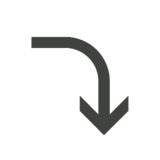
\includegraphics[width=4em]{./arrow.png}

\includebookandcover{evans2003}
\includebookandcover{vernon2013}
\includebookandcover{millett_tune2015}
\end{frame}

%%%%%%%%%%%%%%%%%%%%%%%%%%%%%%%%%%%%%%%%%%%%%%%%%%
\begin{frame}[fragile]{\de{Bücher: Domain-Driven Design allgemein}\en{Resources: Domain-Driven Design in general}}

\includebookandcover{vernon2016}
\includebookandcover{lilienthal_schwentner2017}
\includebookandcover{wlaschin2018}
\end{frame}


%%%%%%%%%%\dir %%%%%%%%%%%%%%%%%%%%%%%%%%%%%%%%%%%%%%%%
\begin{frame}[fragile]{\de{}\en{Want more?}}

{\large
In-depth session on Fri/Sat if interested 
}

\end{frame}
